\documentclass[ht]{article}
\usepackage[a4paper, total={6in, 8in}]{geometry}
\usepackage{booktabs}
\usepackage{multicol}
\usepackage[sorting=none,sortcites=true,backend=bibtex]{biblatex}
\bibstyle{numeric-comp}
\bibliography{bibliography}

\newcommand{\todo}[1]{{\color{red}[\textit{TODO: #1}]}}

\usepackage{tikz}
\usetikzlibrary{calc}
\usetikzlibrary{shapes.geometric, arrows, fit}

\tikzstyle{process} = [rectangle, 
minimum width=12cm, 
minimum height=1cm, 
text width=11cm, 
draw=black, 
fill=white,
rounded corners]

\tikzstyle{subprocess} = [rectangle, 
minimum width=5cm, 
minimum height=0.6cm, 
text centered, 
text width=5cm, 
draw=black, 
fill=white]

\tikzstyle{lsnode} = [rectangle, 
minimum width=2cm, 
minimum height=0.6cm, 
text centered, 
text width=2cm, 
draw=black, 
fill=white]

\tikzstyle{arrow} = [thick,->,>=stealth]
\tikzstyle{dashedarrow} = [dashed,->,>=stealth]

\title{Integrated Vehicle and Crew Planning of Electric Busses using Lagrangian Relaxation and Battery Degredation}
\date{July 2025}
\author{Thomas van der Plas, Han Hoogeveen, Philip de Bruijn}
\begin{document}
\maketitle

\section{Introduction}
Electrification of public transport has become the norm over recent years. Many
public transport poviders, such as the Dutch bus provider Qbuzz
\cite{qbuzzQbuzz}, have been replacing traditional vehicles with electric
vehicles (EVs) in their fleet with the aim of reducing their carbon footprint
in order to match the stricter regulations set out by organizations such as the
European Union \cite{europaRegulation20181999}. This electrification introduces
new challenges in every step of the planning process as laid out in Figure
\ref{fig:planning-overview}. The limits of both electric infrastructure and
electric vehicles add new constraints to an already complex operation. Existing
techniques that minimize operational costs are therefore being revised in order to take into account these operational constraints \todo{beter formuleren}. \\\\ In this work, we
will focus on incorporating electric vehicle restrictions two of the highest operational cost steps in the planning process: vehicle scheduling and crew
scheduling. Crew scheduling in particular is of great importance, as crew costs make
up a majority of the overall operational costs. A recent estimate puts crew
costs at circa $60\%$ of the total operational costs for bus companies in
Northern Europe \cite{Perumal2019Crew}. The set of feasible crew schedules is
however directly influenced by the routes that are determined while planning
vehicles. It has therefore long been known that integrating the vehicle and
crew planning operations can lead to significant reductions in costs, as routes
can be better tailored to suit crew planning needs \cite{Bodin1983}. \\\\ We
will now give an informal overview of the problems at hand. A more formal
overview can be found in Section \ref{sec:problem_def}. The Vehicle Scheduling
Problem (VSP) aims to find a set of minimum cost vehicle tasks such that all
trips that need to be driven throughout a timeperiod are covered. In this, a
trip is defined as full or partial travel of a vehicle along a predetermined
route, and a vehicle task is defined as a set of sequential operations that a
vehicle will perform. Note that for the same route, multiple trips might be
present on a single day if that route is scheduled multiple times. \\ Given a
set of these trips, a set of depots and a set of vehicles, the goal is to find
a vehicle task (or schedule) for each of the vehicles throughout the day. In
this, a task for an individual vehicle must start at a depot, perform a number
of compatible trips (that is, trips which can be performed sequentially while
respecting driving times between trips), before finally returning to its
original depot. In order to minimize operational costs, both the number of
vehicles and the overall driven distance between trips (also called deadheads)
need to be minimized. \\ The VSP with a single depot and unconstrained vehicle
ranges can be solved in polynomial time \cite{Freling2003SDVSP}. The
multi-depot variant of the problem on the other hand is known to be NP-hard
\cite{Bodin1983, Bertossi1987, Even1975}, and the addition of constrained
vehicle ranges such as those found in EVs also make the problem NP-hard
\cite{Bodin1983, Sassi2014}. We consider a general depot case with constrained
vehicle ranges due to the inclusion of EVs, and will therefore refer to the VSP
as being NP-Hard. \\
\\\\ The Crew Scheduling Problem (CSP) on the other hand aims to find a minimum
cost assignment of crew members to vehicle tasks. Given a set of vehicle tasks
and crew members, the goal is to find an assignment of crew members such that
each vehicle is always driven by exactly one driver. In this, constraints such
as maximum working time on a day, driver breaks and handovers between different
drivers on the same vehicle need to be considered. The primary goal for
minimization here is the total amount of workers needed and hours worked. The
CSP is also known to be an NP-hard problem \cite{Fischetti1989}.\\ \todo{Info
  over oplossingen} \\\\ 
As can be seen, the VSP and CSP are closely related. The
vehicle schedules that are selected in the VSP directly determine what crew
assignments are possible within the CSP. It is therefore not always optimal to
fully minimize costs in the vehicle scheduling process, as this might incur
higher overall costs due to crew scheduling. We can therefore roughly split the solving of vehicle and crew assignments into two seperate approaches: sequential, in which the VSP and CSP are solved seperately, or integrated, in which the VSP and CSP are solved such that overall costs are minimized simultaniously. The integrated approach is often
refered to as the vehicle and crew scheduling problem, or VSCP. The VSCP can also still be further subdivided into full and partial integration, partial integration adds some additional crew hueristics to the VSP and full integration actually minimizes costs of both. In this work, we will only focus on full integration. \todo{beter formuleren} \\\\ 
A lot of work has already been done for the VSP, CSP and VSCP. Both the sequential and
integrated approach have been extensively studied since the \todo{1980s?}, and
we refer the reader to a recent survey in order to get a sense of the current
state of the art \todo{citiation met survey}. The introduction of electric
vehicles has however introduced new constraints. The most important constraint
is the limited range of electric vehicles, combined with charging times which are
much greater than refeuling times found on traditional combustion based buses. This most
directly effects the VSP, as charging periods now need to be added throughout
the day in order to effectively use buses. This new version of the problem,
refered to as the E-VSP, has also been studied extensively in recent years. We
refer the reader to a survey by Perumal et al. for a detailed overview of
recent progress \cite{Perumal2022LitRev}. \\\\ Most research related to the
scheduling of electric public transport vehicles up until now has focused on
the sequential approach. Limited literature does exist on the E-VSCP problem,
however simplifying assumptions are made which might limit real world
applicability or accurate modeling of costs. Most notably, assumptions are made
about charging locations (such as only being able to charge at a bus depot) or
charging behavior (such as modeling the process as being purely linear or only
allowing full charges). Additionally, to the best of our knowledge battery
degredation due to usage patterns has not been included in any integrated
models at the time of writing. The contribution of this work is therefore
threefold:
\begin{itemize}
  \item Incorporating nonlinear battery charging times.
  \item Including battery degredation due to usage patterns into the objective function.
  \item Using Lagrangian relaxation in order to link the VSP and CSP instead of currently used methods.
\end{itemize}
This work is organised as follows. In Section 2, we will discuss work related to the E-VSCP and give an overview of common ways of modeling the problem. In Section 3, we give our formal problem definition. \todo{uitbreiden zodra je meer info hebt}.
\begin{figure}[h]
  \centering
  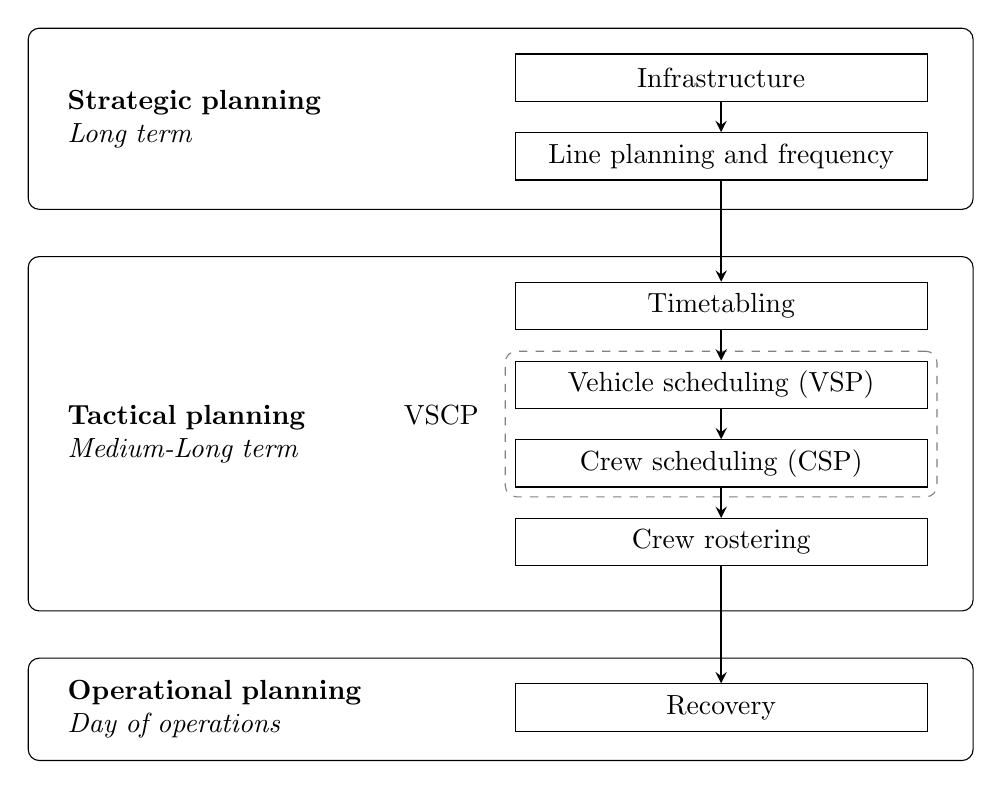
\begin{tikzpicture}[node distance=2cm]
    \node (strategic) [process, minimum height=2.3cm] {\textbf{Strategic planning}\\\textit{Long term}};
    \node at (strategic.base) (infra) [subprocess, xshift=2.8cm, yshift=0.4cm] {Infrastructure};
    \node at (strategic.base) (line) [subprocess, below of=infra, yshift=1cm] {Line planning and frequency};

    \node (tactical) [process, minimum height=4.5cm, below of=strategic, yshift=-2cm] {\textbf{Tactical planning}\\\textit{Medium-Long term}};
    \node at (tactical.base) (timetable) [subprocess, xshift=2.8cm, yshift=1.5cm] {Timetabling};
    \node at (tactical.base) (vehicle) [subprocess, below of=timetable, yshift=1cm] {Vehicle scheduling (VSP)};
    \node at (tactical.base) (crew) [subprocess, below of=vehicle, yshift=1cm] {Crew scheduling (CSP)};
    \node at (tactical.base) (vscp) [rounded corners, dashed, draw=gray, fit=(vehicle) (crew), align=left] {\hspace{-4em}VSCP};
    \node at (tactical.base) (rostering) [subprocess, below of=crew, yshift=1cm] {Crew rostering};

    \node (operational) [process, minimum height=1.3cm, below of=tactical, yshift=-1.5cm] {\textbf{Operational planning}\\\textit{Day of operations}};
    \node at (operational.base) (recovery) [subprocess, xshift=2.8cm, yshift=-0.1cm] {Recovery};

    \draw [arrow] (infra) -- (line);
    \draw [arrow] (line) -- (timetable);
    \draw [arrow] (timetable) -- (vehicle);
    \draw [arrow] (vehicle) -- (crew);
    \draw [arrow] (crew) -- (rostering);
    \draw [arrow] (rostering) -- (recovery);
  \end{tikzpicture}
  \caption{A general overview of the public transport planning process, based on \cite{Ceder1986, Ibarra-Rojas2015, Perumal2022LitRev}.}
  \label{fig:planning-overview}
\end{figure}

\begin{table}[h]
  \centering
  \begin{tabular}{ll}
    \toprule
    \multicolumn{1}{l}{\textbf{Abbreviation}} & \multicolumn{1}{l}{\textbf{Definition}}               \\
    \cmidrule(lr){1-1}\cmidrule(lr){2-2}
    ALNS                                      & Adaptive Large Neighbourhood Search                   \\
    B\&P                                      & Branch-and-Price                                      \\
    CG                                        & Column Generation                                     \\
    CSP                                       & Crew Scheduling Problem                               \\
    E-\dots                                   & Problem \dots with electric vehicles                  \\
    LNS                                       & Large Neighbourhood Search                            \\
    LS                                        & Local Search                                          \\
    MDVSP                                     & Multi Depot Vehicle Scheduling Problem                \\
    MIP                                       & Mixed Integer Program                                 \\
    SAA                                       & Simulated Annealing Algorithm                         \\
    SDVSP                                     & Single Depot Vehicle Scheduling Problem               \\
    SoC                                       & State of Charge                                       \\
    TCO                                       & Total Cost of Ownership                               \\
    ToU                                       & Time of Usage                                         \\
    TVSP                                      & Integrated Timetabling and Vehicle Scheduling Problem \\
    VCSP                                      & Integrated Vehicle and Crew Scheduling Problem        \\
    VSP                                       & Vehicle Scheduling Problem                            \\
    \bottomrule
  \end{tabular}
  \caption{Nomenclature used in this work}
\end{table}

\section{Related work}
In this section, we will discuss work related to our research into the E-VSCP.
An overview of how batteries and charging behavior is modeled in different
E-VS(C)P approaches has also been included in Table \ref{tab:evscp-lit}. \\\\
\noindent \textbf{(E-)VSP} \\\\ \todo{modeleer methode toevoegen}\\ The SDVSP
has long been known to be polynomially solvable, however the inclusion of
multiple depots has been shown to make the problem NP-hard under the assumption
that busses must return to the same depot from which they originated
\cite{Bunte2009}. Additionally, the introduction of any resource constraints
such as limited ranges within the VSP has also been
shown to be NP-hard by Bodin et al. \cite{Bodin1983}. As the E-VSP deals with
the limited range associated with electric vehicles, it is quite closely
related to the multiple depot vehicle scheduling problem with route time
constraints (MDVSP-RTC) \cite{Haghani2002}. The key difference between these
two problems is that the E-VSP allows for (partial) recharging of a vehicle
throughout the operating period, whereas the MDVSP-RTC assumes a fixed maximum
travel time for the vehicle within the given period. The E-VSP specifically
been shown to be NP-hard by Oulamara and Sassi \cite{Sassi2014}. \\\\

Li was one of the first to consider the E-VSP back in 2014 \cite{Li2014}. The
model is based on an extension of the traditional network based approach to
solving the VSP, with the additional constraint of total driving time. It
additionally assumes that fast charging or battery swaps are possible, ensuring
full charges in a fixed timespan. The model is solved using a column generation
approach with branch-and-price, followed by a local search to find a local
optimum. The proposed methods are tested on trips in the San Fransisco Bay Area, with a
maximum instance size of 242 trips. These tests resulted in optimality gaps of
$<5\%$ for busses able to drive 150km, and between 7-15\% for a range of 120km
depending on the instance. \\\\

\todo{meer info} van
Kooten Niekerk et al. introduce a pair of models which aim to solve the E-VSP
while taking into account ToU energy prices, nonlinear charging times and
battery degredation due to depth of discharge \cite{vanKootenNiekerk2017}. They
do this by extending the graph underlying the traditional VSP using either
continuous or discrete state of charge variables for the trip nodes,
and solve using CG. They test using data provided
by Belgian bus company De Lijn in the city Leuven, using a total of 543 trips. They show that the
discretized model can be solved in a shorter timeframe with similar results to
the continuous model. \\\\

Jiang et al. use a LNS approach to solve the E-VSP \cite{Jiang2021}. They
consider time of use energy costs and opportunisitic charging. They use test
data in Shenzhen, China with a total of 778 trips. \todo{meer info maar de
  paper is saai}.\\\\

De Vos et al. introduce an E-VSP solution method which deals with partial
recharges and capacitated charging stations \cite{deVos2024}. They model this
using discrete battery charge levels in a connection-based network of trips and
charging actions, in which a primal network is created using pessemistic
rounding. In order to solve, they apply CG with two seperate hueristics:
branch-and-price and a diving hueristic. To overcome the limitations of dual
bounds resulting from a discretized model, they incorporate ideas from Boland
et al. resulting in a dual network with optimistic connections
\cite{Boland2017}. This gives the same bounds as the ones found in the
non-discretized model. Testing is performed on a bus concession south of
Amsterdam with 816 trips, with subsets being used as smaller instances.
Optimality gaps of 1.5-2.7\% are achieved across instances. They additionally
note that the framework as provided can easily be extended for nonlinear
charging functions and depth-of-discharge battery degredation. \\\\

Olsen and Kliewer introduce a solution to the E-VSP which aims to incorporate
more accurate nonlinear charging times \cite{Olsen2020}. They focus on showing
that a linear approximation for the second phase of vehicle charging (such as
the one found in van Kooten Niekerk \cite{vanKootenNiekerk2017}) can
misrepresent the SoC and required charging times, and therefore advocate for
the use of an exponential function to model this phase instead. \\\\

Parmentier et al. consider a scalable approach to the E-VSP which is based on
the concept of nondominated charging arcs with nonlinear charging
\cite{Parmentier2023}. They use these in order to formulate a more
computationally efficient version of the pricing problem given uniform charging
infrastructure. Using CG and B\&P techniques, they test on the \textit{large}
instances introduced by Wen et al. \cite{Wen2016} which included up to 8
depots, 16 charging stations and 500 trips. Here, they are able to find
solutions that are only up to 0.06\% away from the optimum. \\\\

Pulyassary et al. show that the E-VSP is solvable in polynomial time given the
assumption that the shortest path between two trips in the flow network is
equal to the path with lowest battery usage \cite{Pulyassary2024}. They
consider the case in which charging at a select number of capacity bound nodes
is allowed with nonlinear charging behavior. For the single depot case, a
$O^*(|T|^6)$ algorithm for finding a set of vehicle schedules with lowest cost
given trips $T$ is provided based on DP. Additionally, polynomial algorithms
for determining maximum feasible charging capacity and minimum-cost flows based
on LP are provided. No computational experiments are performed. \\\\

Zhang et al. apply a similar method to the one found in van Kooten Niekerk
\cite{Zhang2021}. They consider a single depot with charging infrastructure,
where multiple round trip lines originating from the depot. They model
nonlinear charging behavior, battery depreciation due to depth of discharge and
capacitated charging infrastructure using discretized timesteps. They solve
using a combination of CG and B\&P. Tests are done on both randomly generated
instances as well as 6 not yet electrified lines with up to 160 and 197 trips
respectively. Cost savings of 10.1–27.3\% in the real life line based on
different battery capacities. \todo{waar de fuck vergelijken ze mee}
\todo{Bekijken} multidepot multivehicle type esvp, multi-commodity flow,
proximal bundle method https://epubs.siam.org/doi/10.1137/040603929
\todo{lezen}\cite{Borndörfer2024}

\todo{grafiek elektrificatie bussen in NL}

\noindent \textbf{(E-)CSP}\\
The CSP is often solved as a set partitioning (or set covering) problem. Here, the tasks described by the sequences of trips generated during the VSP must be covered by the individual schedules of crew members. Research into this subject is primarily done in the airline space; crew costs here are generally even higher than those found in the more general public transport sector \cite{Barnhart2003}. Additionally, strong labor unions and restrictive labor legislation due to safety concerns cause a large number of constraints to be applied to crew schedules, resulting in a non-trivial problem to solve. \\
Results achieved in the aviation space quite easily generalize to other sectors, and we will therefore discuss some of note. For a more detailed overview, we refer the reader to a recent review by Deveci and Demirel \cite{Deveci2018}. \\\\
\todo{https://www.sciencedirect.com/science/article/pii/S2352146517301643}
  
\todo{modeleer methode toevoegen}\\

\noindent \textbf{(E-)VSCP}\\
\todo{Normale VSCP}\\
As far as we are aware, at the time of writing only five other works discuss the fully integrated E-VSCP. \\\\

Perumal et al. were the first to offer a solution to the E-VSCP in 2021
\cite{Perumal2021}. They introduced an ALNS which incorporates a B\&P hueristic
which has been previously used to solve the MDVSP, E-VSP and VCSP
\cite{Pepin2009, Haase1996, vanKootenNiekerk2017}. Additionally, they adapt an
embedding of a B\&P hueristic into the ALNS as introduced by Pepin et al.
\cite{Pepin2009}. They only consider full recharges with a fixed duration of
120 minutes, charging at the depot and fixed maximum ranges for vehicles. The
authors tested using real life data from lines in Denmark and Sweden with a
maximum instance size of 1109 trips, and report an improvement of $1.17-4.37\%$
across different instances when compared to a sequential approach. \\\\

Sistig and Sauer also offered a ALNS based approach in 2023, which aimed to
improve upon the approach presented by Perumal et al. by including partial
recharges, opportunisitic charging at terminal stops of trips and non-fixed
ranges for the vehicles \cite{Sistig2023}. In order to solve, they implement a
selection of 3-step ALNS neighborhoods consisting of E-VSP modification,
finding a solution to the corresponding CSP and consequently modifying the CSP
solution. Tests were done using an instance of a city route in Germany, with a
total of 282 trips. Different scenarios based on possible crew break and relief
locations were considered in order to compare diesel and electric TCO.
Additionally, sensitivity analysis of the TCO was done for parameters such as
electricity, driver and fixed costs. \\\\

Wang et al. introduce a two layered model using particle swarms and a
$\epsilon$-constraint based mechanism which allows for a mix of traditional
combustion and electric busses \cite{Wang2022}. The model incorporates partial
depot charging, as well as measures to ensure that crew is primarily assigned
the same vehicle throughout the day. A circular bus route in Changchun, China
with 68 daily trips is used as a basis for testing, with a focus on electric
versus diesel usage and driver satisfaction. \\\\

Shen and Li provide a minimum-cost flow framework for the E-VSP which is
integrated with a set partitioning based approach for the E-CSP
\cite{Shen2023}. They only provide full recharge capabilities at the depot,
however focus on the inclusion of a distinction between driving and standstill
time of vehicles in order to more accurately model real life traffic. A city
line in China with 270 daily trips is used for testing, resulting in cost
savings of up to 8.7\% when compared to a sequential approach. \\\\

Cong et al. provide a hybrid MIP and SAA based approach to optimizing a mixed
fleet of combustion and electric vehicles with ToU electricity pricing
\cite{Cong2024}. In each SAA iteration, a collection of new E-VSP trip
assignments are created using neighborhood operations, after which two MIP
models are sequentially employed to solve for charging and crew schedules. The
methods are tested on a collection of 3 bus routes originating from the same
depot in Changchun City, China with a total of 520 trips across all routes.
When compared to the sequential approach, the integrated vehicle schedule was
able to reduce costs by 0.8\%. \todo{miss nog iets zeggen over hoe ze dit eerst
  hadden ingesteld} \\\\

\noindent \textbf{Other related fields}\\
The VSP is also very closely related to the vehicle routing problem (VRP). The VRP with time windows is of particular interest, as this allows us to define the same precedence constraints as those naturally defined by trips. \todo{Uitbreiden met papers, betere beschrijving}
\todo{Meer related werk: }
\todo{E-VRPTWR}
Research has also been done into integrating the E-VSP with timetable planning (E-TVSP). A recent example can be found in the work of Stadnichuk et al., who allowed results of the E-VSP to introduce optimality cuts into the MIP used for creating timetable plans as a way to reduce costs \cite{Stadnichuk2024}. This is achieved by transforming the E-VSP problem into one of bin packing with conflicts, after which three different hueristic methods are applied and compared. \todo{iets beter formuleren allemaal}. \\\\

\begin{table}[h]
  \centering
  \begin{tabular}{clllllll}
    \toprule
                                     & Model  & ToU & SoC & Nonlinear Ch. & Partial Ch. & Ch. Location & Degredation \\
    \cmidrule(lr){2-8}
    \cite{Li2014} 2014               & E-VSP  & No  & D   & No            & No          & D            & No          \\
    \cite{vanKootenNiekerk2017} 2017 & E-VSP  & Yes & C/D & Yes           & Yes         & D/O          & Yes         \\
    \cite{Olsen2020} 2020            & E-VSP  & No  & C   & Yes           & Yes         & D/O          & No          \\
    \cite{Jiang2021} 2021            & E-VSP  & Yes & C   & No            & Yes         & O            & No          \\
    \cite{Zhang2021} 2021                 & E-VSP  & No  & C/D & Yes           & Yes         & D            & Yes \\
    \cite{Parmentier2023} 2023       & E-VSP  & No  & C   & Yes           & Yes         & D/O          & No          \\
    \cite{deVos2024} 2024            & E-VSP  & No  & D   & Yes           & Yes         & D/O          & No          \\
    \cite{Pulyassary2024} 2024       & E-VSP  & No  & C/D & Yes           & Yes         & O            & No          \\
    \addlinespace[0.4em]
    \cite{Perumal2021} 2021          & E-VSCP & No  & C   & No            & No          & D            & No          \\
    \cite{Sistig2023} 2023           & E-VSCP & No  & C   & No            & Yes         & D/O          & No          \\
    \cite{Wang2022} 2022             & E-VSCP & Yes & C   & No            & Yes         & D            & No          \\
    \cite{Shen2023} 2023             & E-VSCP & No  & C   & No            & No          & D/O          & No          \\
    \cite{Cong2024} 2024             & E-VSCP & Yes & C   & No            & Yes         & D            & No          \\
    \addlinespace[0.4em]
    \cite{Stadnichuk2024} 2024       & E-TVSP & No  & C   & No            & Yes         & D/O          & No          \\
    \bottomrule
  \end{tabular}
  \caption{A brief overview of battery modeling in E-VSCP related literature. SoC modeled as (D)iscrete or (C)ontinuous variable, Charge locations at (D)epot, (T)erminal trip stops, (I)n motion, Degredation of battery in cost function}
  \label{tab:evscp-lit}
\end{table}

\section{Problem definition}
\label{sec:problem_def}
Let $T$ be a set of trips that needs to be run.


\todo{csp bus variant}
\todo{E-VRPTWRC}
\todo{Inkorten wat niet interessant is}
\todo{onderzoeksgat}
\printbibliography
\end{document}